\chapter{Requirements Elicitation}

% https://uim.fei.stuba.sk/wp-content/uploads/2018/02/Object-oriented-Software-Engineering-3rd-Edition.pdf

% \textit{Note: This chapter follows the Requirements Analysis Document Template in \cite{bruegge2004object}. 
% \textbf{Important:} Make sure that the whole chapter is independent of the chosen technology and development platform. The idea is that you illustrate concepts, taxonomies and relationships of the application domain independent of the solution domain!
% Cite \cite{bruegge2004object} several times in this chapter.}

This chapter follows the Requirements Analysis Document Template based on Bernd Bruegge's \textit{Object Oriented Software Engineering Using UML, Patterns, and Java} \cite{bruegge2004object}. 
The goal is to illustrate the concepts, taxonomies, and relationships of the application domain independent of the chosen technology and development platform. 
The following sections provide an overview of the system, describe functional and nonfunctional requirements, and outline important system models.

\section{Overview}

% \textit{Note: Provide a short overview about the purpose, scope, objectives and success criteria of the system that you like to develop.}

The system being developed has the purpose of collecting typing pattern of its users with the purpose of inferring their age group by analysing their typing patterns.
Potential future improvements of the application include the addition of real-time analysis and result.
It is also possible to use the system to gather the data for follow-up research on detecting early signs of neurodegenerative diseases with typing pattern.
These potential future improvements are, however, beyond the scope of this thesis.

The system's primary objectives are to collect, process and save keystroke data efficiently, so that the data can be analysed.
To achieve this, the application also needs to provide a condusive condition for the users, so that they are able to type as they usually would.
This means that the application would need to integrate and prompt the \ac{LLM} to elicit response from the users.
The \ac{LLM} will be prompted to elicit as many response from the users as possible, so that more data can be gathered and the analysis can be more accurate.

User experience is also an important part of the application.
The user should feel comfortable using the application as they would usually use another chatting application.
Accessibility, especially for the elderly users, needs to be taken into account.
This is important to make sure that differences in typing pattern are only caused by internal factors of the user themselves.
Success of this application will be measured by the ability of the system to gather, process and save keystroke data accurately and effectively.

\section{Requirements}

% \textit{Note: If you leave out the section ``Current system'', you can rename this section into ``Requirements''.}

The application will provides a condusive condition for the user to type.
Typing pattern of the user will be collected, processed and saved in the database for later to be analyzed.
The proposed system will be split into functional and nonfunctional requirements.

\subsection{Functional Requirements}

% \textit{Note: List and describe all functional requirements of your system. Also mention requirements that you were not able to realize. The short title should be in the form ``verb objective''}

The functional requirements (FR) define the specific actions that the system must perform. 
Below is a list of the primary functional requirements:

\begin{itemize} 
    \item [FR1] \textbf{Condusive Typing Environment}: The user should feel comfortable using the system, as they would using other chatting application.
    \item [FR2] \textbf{Elicite User Response}: The system must be able to elicit response from the users by using \ac{LLM}. 
    \item [FR3] \textbf{Collect Typing Data}: The system must capture and log keystroke data from the user in real time, including keypresses and timestamps. 
    \item [FR4] \textbf{Store Typing Data}: The system must securely store all captured typing data in the database for future analysis. 
    \item [FR5] \textbf{Store Users' Age}: The system must gather users' age to act as a comparison between infered and actual age group of the user. 
    \item [FR6] \textbf{Ensure Data Anonymization}: The system must anonymize user data before analysis to ensure compliance with privacy standards. 
\end{itemize}

\subsection{Nonfunctional Requirements}

% \textit{Note: List and describe all nonfunctional requirements of your system. Also mention requirements that you were not able to realize. Categorize them using the FURPS+ model described in \cite{bruegge2004object} without the category \textbf{functionality} that was already covered with the functional requirements.}

% \begin{itemize}
% \item [NFR1] \textbf{Category}: Short Description.
% \item [NFR2] \textbf{Category}: Short Description.
% \item [NFR3] \textbf{Category}: Short Description.
% \end{itemize}

The nonfunctional requirements (NFR) define system constraints, performance criteria, and standards the system must adhere to. 
These requirements are categorized using the FURPS+ model, as described in Bernd Bruegge's book \cite{bruegge2004object}, excluding functionality, which was covered in the functional requirements section.

\begin{itemize} 
    \item [NFR1] \textbf{Usability and Accessibility}: The user interface must be easy to use, especially for elderly users.
    Design of the application should be accessible for the elderly with features such as large fonts, enough spacing, and clear visual indicators. 
    \item [NFR2] \textbf{Reliability}: The system must be able to run and save users' typing pattern without loss of data or functionality. 
    \item [NFR3] \textbf{Performance}: The system should give response to the user within 10 seconds after the user send a message. 
    \item [NFR4] \textbf{Privacy}:
    The user's information other than their age should be anonym.
    Chat session of users should be able to be locked, so that it cannot be accessed anymore.
    \item [NFR5] \textbf{Adaptability}: The system must be able to scale to support more users, e.g. by adding more servers.
    It should also be possible to add functionalities such as real-time analysis. 
\end{itemize}

Among these requirements, the most challenging to implement is the adaptability and performance requirement.
Adaptability requirement is challenging because it involves the system's ability to scale to support more users and functionalities.
The system must be designed to be scalable and flexible to accommodate future changes and additions.
It is a very time consuming process to design and develop a system that can be easily scaled and adapted to new functionalities.
The development process of the application is unfortunately limited by time, which makes it hard to implement this requirement.

The performance requirement is challenging because it involves the system's ability to respond to user input within 10 seconds.
It is obvious that the respond time is largely dependent on the response time of the \ac{LLM}.
On practice, the \ac{LLM} is able to respond within 10 seconds most of the time.
However, there are times when the \ac{LLM} needs more time to respond, e.g. when the response is long.
One of the way to solve this problem is to implement a streaming system, where the \ac{LLM} can send the response in chunks.
This way, the user can already see the response while the \ac{LLM} is still typing the response.
Here too, the time limitation of the thesis makes it hard to implement this solution.


\section{System Models}

% \textit{Note: This section includes important system models for the requirements analysis.}

This section includes key system models for requirements analysis, including scenarios, use case models, object models, dynamic models, and user interface.

\subsection{Scenarios}

% \textit{Note: If you do not distinguish between visionary and demo scenarios, you can remove the two subsubsections below and list all scenarios here.}
A scenario is “a narrative description of what people do and experience as they try to make use of computer systems and applications” \cite{Carroll1995}. 
The following section will show concrete, focused and informal description of features of the application from the viewpoint of the user. 

\subsubsection{Visionary Scenarios}

% \textit{Note: Describe 1-2 visionary scenario here, i.e. a scenario that would perfectly solve your problem, even if it might not be realizable. use our scenario description template in form of a table.}

The following scenario describes an ideal scenario that might be achieved in a future research.

\begin{longtable}{p{0.2387\textwidth} p{0.7\textwidth}}
    \toprule
    \raggedright \textit{Scenario name} & \closeline{neurodegenerativeDiseaseDetection}\tabularnewline
    \hline
    \endhead
    \raggedright \textit{Participating actor instances} & \raggedright bob: User\tabularnewline
    \hline
    \raggedright \textit{Flow of events}&
    \begin{minipage}[t]{0.7\textwidth}
        \begin{itemize}[noitemsep,leftmargin=*,topsep=0pt,parsep=0pt,partopsep=0pt]
               \item[1.] Bob, a man in his late 50s, use a chatting application to chat with his grandson.
               This chatting application is already integrated with a system to capture and analyze typing pattern.
               \item[2.] Even though Bob does not notice it at all, the application records his typing pattern while simultaneously analysing it.
               After some times, the application notifies Bob that the system has detected with 90\% certainty early symptoms of \ac{AD} on Bob.
               Bob then seeks medical help to confirm this analysis.
       \end{itemize}
    \end{minipage}
    \tabularnewline
    \bottomrule
    \caption{Neurodegenerative diseases detection using typing pattern analysis}
    \label{neurodegenerativeDiseaseDetection}
\end{longtable}

\subsubsection{Demo Scenarios}

% \textit{Note: Describe 1-2 demo scenario here, i.e. a scenario that you can implement and demonstrate until the end of your thesis. use our scenario description template in form of a table.}

The following scenario is implemented by the current system.
It is the main purpose and functionality of the application. 

\begin{longtable}{p{0.2387\textwidth} p{0.7\textwidth}}
    \toprule
    \raggedright \textit{Scenario name} & \closeline{ageGroupDetection}\tabularnewline
    \hline
    \endhead
    \raggedright \textit{Participating actor instances} & \raggedright bob: User\tabularnewline
    \hline
    \raggedright \textit{Flow of events}&
    \begin{minipage}[t]{0.7\textwidth}
        \begin{itemize}[noitemsep,leftmargin=*,topsep=0pt,parsep=0pt,partopsep=0pt]
               \item[1.] Bob, a man in his late 50, uses the application to chat with a \ac{LLM}.
               The application logs and stores Bob's keystrokes. 
               \item[2.] This keystrokes data is then later analyzed.
               After the analysis is done, it is correctly inferred that Bob is in the age group of 50 to 60 years old.
       \end{itemize}
    \end{minipage}
    \tabularnewline
    \bottomrule
    \caption{Age group detection using typing pattern analysis}
    \label{ageGroupDetection}
\end{longtable}

\subsection{Use Case Model}

% \textit{Note: This subsection should contain a UML Use Case Diagram including roles and their use cases. You can use colors to indicate priorities. Think about splitting the diagram into multiple ones if you have more than 10 use cases.
% \textbf{Important:} Make sure to describe the most important use cases using the use case table template. Also describe the rationale of the use case model, i.e. why you modeled it like you show it in the diagram.}

The following use case model show the interactions between the user, the server and the \ac{LLM}. 

\begin{figure}[h!]
    \centering
    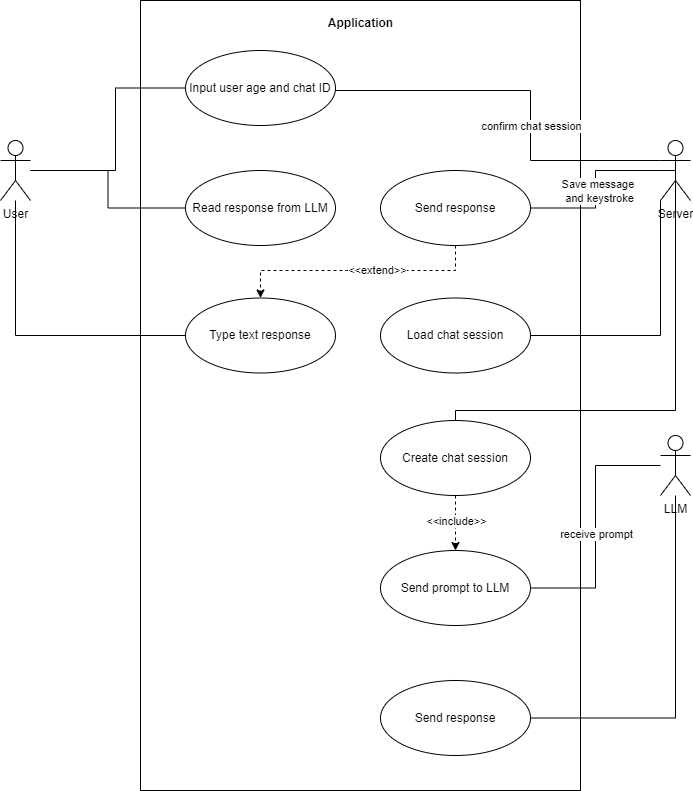
\includegraphics[width=13cm]{usecase}
    \caption{UML use case diagram of the chatting feature}
\end{figure}

\begin{longtable}{p{0.2387\textwidth} p{0.7\textwidth}}
\toprule
\raggedright \textit{Use case name} & initialization of chat session. \tabularnewline
\hline
\endhead
\raggedright \textit{Participating actors} & Initiated by user. \newline Communicates with server and \ac{LLM}. \tabularnewline
\hline
\raggedright \textit{Flow of events} & \begin{minipage}[t]{0.7\textwidth}
	\leftenum{1.}{User inputs age and chat ID.}
	\rightenum{2.}{Backend server confirms that the ID is valid and accessible.}
	\rightenum{3.}{Backend server checks that no corresponding session with this ID has been created and initialises a new chat session.}
	\rightenum{3.}{Backend server gives a prompt to \ac{LLM}.}
	\leftenum{4.}{\ac{LLM} loads and send the first message after it is finished loading.}
	\rightenum{5.}{User reads the message from the \ac{LLM}}

\end{minipage}
\smallskip\tabularnewline
\hline
\raggedright \textit{Entry condition} & \shortitem{0.7\textwidth}{\item User opens the login page of the application.}\tabularnewline
\hline
\raggedright \textit{Exit condition} & \shortitem{0.7\textwidth}{\item  User reads the first message from the \ac{LLM}.}
\smallskip\tabularnewline
\hline
\raggedright \textit{Quality requirements} & \shortitem{0.7\textwidth}{
    \item The server should be able to checks that the corresponding chat of the given ID is accessible and has no chat history.
    \item The server should initialise the chat session correctly and save the age user data corresponding to this chat session in the database.
    \item The server should send a prompt to the \ac{LLM}, wait for the response, and forward the response of the \ac{LLM} to the user.
    }\tabularnewline
 \bottomrule
\caption{Use case initialization of chat session}
\label{useCaseInitialization}
\end{longtable}

\begin{longtable}{p{0.2387\textwidth} p{0.7\textwidth}}
    \toprule
    \raggedright \textit{Use case name} & loading of an already existing chat session. \tabularnewline
    \hline
    \endhead
    \raggedright \textit{Participating actors} & Initiated by user. \newline Communicates with server and \ac{LLM}. \tabularnewline
    \hline
    \raggedright \textit{Flow of events} & \begin{minipage}[t]{0.7\textwidth}
        \leftenum{1.}{User inputs age and chat ID.}
        \rightenum{2.}{Backend server confirms that the ID is valid and accessible.}
        \rightenum{2.}{Backend server checks that there exists already a chat session with the corresponding ID.}
        \rightenum{3.}{Backend server loads all the messages history of this chat session and sends it to the user.}
        \leftenum{4.}{User reads the chat history and continues the chat as they left it.}
    
    \end{minipage}
    \smallskip\tabularnewline
    \hline
    \raggedright \textit{Entry condition} & \shortitem{0.7\textwidth}{\item User opens the login page of the application.}\tabularnewline
    \hline
    \raggedright \textit{Exit condition} & \shortitem{0.7\textwidth}{\item  User is able to read all of the chat history belonging to the session with the ID given by the user.}
    \smallskip\tabularnewline
    \hline
    \raggedright \textit{Quality requirements} & \shortitem{0.7\textwidth}{
    \item The server should be able to checks that the corresponding chat of the given ID is accessible and has chat history.
    \item The server should load all chat history of this chat session correctly.
    \item The server should send the chat history data to the user with right information of whether a message is sent by the user or by the \ac{LLM}.
    }\tabularnewline
    \bottomrule
    \caption{Use case loading of an alredy existing chat session}
    \label{useCaseLoading}
\end{longtable}

\begin{longtable}{p{0.2387\textwidth} p{0.7\textwidth}}
    \toprule
    \raggedright \textit{Use case name} & user sends a message. \tabularnewline
    \hline
    \endhead
    \raggedright \textit{Participating actors} & Initiated by user. \newline Communicates with server and \ac{LLM}. \tabularnewline
    \hline
    \raggedright \textit{Flow of events} & \begin{minipage}[t]{0.7\textwidth}
        \leftenum{1.}{User types a response to the last message from the \ac{LLM}.}
        \leftenum{2.}{User sends the message.}
        \rightenum{3.}{Backend server saves the message and its keystroke data in the database.}
        \rightenum{4.}{Backend server sends the message to the \ac{LLM}.}
        \leftenum{5.}{\ac{LLM} responses to the user's message.}
        \rightenum{6.}{Backend server saves the message from the \ac{LLM} in the database and sends it to the user.}
    
    \end{minipage}
    \smallskip\tabularnewline
    \hline
    \raggedright \textit{Entry condition} & \shortitem{0.7\textwidth}{\item User is already in a chat session.}\tabularnewline
    \hline
    \raggedright \textit{Exit condition} & \shortitem{0.7\textwidth}{\item  User is able to read the message from the \ac{LLM}.}
    \smallskip\tabularnewline
    \hline
    \raggedright \textit{Quality requirements} & \shortitem{0.7\textwidth}{
    \item The server should save the message from the user and its keystroke data in the database correctly.
    \item The server should forward the message to the \ac{LLM}.
    \item The server should wait for the \ac{LLM} to response, . 
    }\tabularnewline
    \bottomrule
    \caption{Use case user sends a message}
    \label{useCaseSendMessage}
\end{longtable}

\subsection{Analysis Object Model}

% \textit{Note: This subsection should contain a UML Class Diagram showing the most important objects, attributes, methods and relations of your application domain including taxonomies using specification inheritance (see \cite{bruegge2004object}). 
% Do not insert objects, attributes or methods of the solution domain.
% \textbf{Important:} Make sure to describe the analysis object model thoroughly in the text so that readers are able to understand the diagram. 
% Also write about the rationale how and why you modeled the concepts like this.}

The following diagram shows the key objects and their relations with other objects in the application.

\begin{figure}[h!]
    \centering
    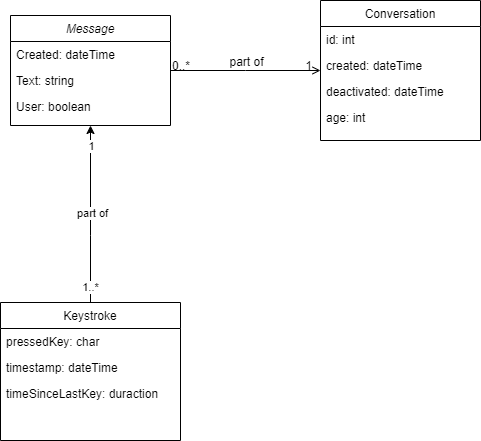
\includegraphics[width=13cm]{classuml}
    \caption{UML class diagram of the application domain}
\end{figure}

\textbf{Classes}: Message, Conversation, Keystroke

Conversation: Represents the whole chatting session with a unique ID.
When the user enters an ID, the backend server will look for a conversation that has the same ID.
If such object exists, then the server will fetch the conversation along with the Messages that belong to this conversation object.
If the object does not exist, then the server will initialise a new conversation object with ID that just has been given by the user.
Each conversation object also has age attribute, which give information about the age of the user to whom this object belongs to.
To improve privacy, each conversation is also given the attribute deactivated.
If this attribute is set, then the conversation will not accessible anymore.
This helps prevent unwanted actors to access chat sessions of users that are already finished.

Message: Represents each message that the user or the \ac{LLM} sent.
Each message object is related to one conversation.
Whereas each conversation contains between zero and multiple messages.
The messages from the \ac{LLM} also need to be saved, so that the whole conversation can be loaded again, after the user exits a chat session.
As a result, the message objects need to have an attribute to give information, whether this message was created by the user or by the \ac{LLM}.
This information is saved in the boolean attribute "user".

Keystroke: Represents each keystroke that the user types.
Each message object will have between one and multiple keystrokes.
The keystroke object is the most important object for this thesis, since the reseach will be focused on the keystrokes of the user.
Each keystroke object will have three attributes: pressedKey, timestamp, and timeSinceLastKey.
Each key the user pressed will be saved as a keystroke object, such as alphabets, numbers, and control characters, such as backspace or horizontal tab.
This information is saved on the attribute pressedKey.
The attribute timeSinceLastKey will show the duration between each key presses.
Statistical analysis of the keystrokes will be based on the value saved on the attribute timeSinceLastKey. 

\subsection{Dynamic Model}

% \textit{Note: This subsection should contain dynamic UML diagrams. These can be a UML state diagrams, UML communication diagrams or UML activity diagrams.\textbf{Important:} Make sure to describe the diagram and its rationale in the text. \textbf{Do not use UML sequence diagrams.}}

Figure~\ref{state} depicts UML state diagram of the application.
This diagram shows the states the application will be in based on certain triggers.
The entry point of the application would be the login page.
This will be the first page the user accessed.
If the user inputted the correct ID, i.e. accessible ID with the right format, then the second condition will be checked.
If the ID is not correct, then a warning will be shown.

The second condition consists of checking whether the chat session corresponding to the ID has been initialised.
An initialised chat session means that the chat session has already been accessed before.
This chat session possibly already has chat history that needs to be loaded.
If, on the other hand, the entered ID is not associated with any chat session, this means that this is the first time the user entered this ID.
In this case, the chat session needs to be initialised first.
After the chat session is initialised, then a prompt is given to the \ac{LLM}.
The first message from the \ac{LLM} is then sent to the user.

After either the first message from the \ac{LLM} or the whole chat history of the chat session is loaded, the application enters the next state.
In this state, the application waits for the user to type and send the message.
Message that is sent by the user is then processed in the backend server.
To begin with, the message is sent to the \ac{LLM}.
The server then waits for the \ac{LLM} to respond to the text.
It should be mentioned here that the server sends the whole chat history to the \ac{LLM}, so that the context of the previous messages is not lost.
After the \ac{LLM} responded, both the new message from the user and from the \ac{LLM} are then saved in the database.
In the end, the new message from the \ac{LLM} is forwared to the user.
This bring the application back to the state of waiting for the user to send a message.

\begin{figure}[h!]
    \centering
    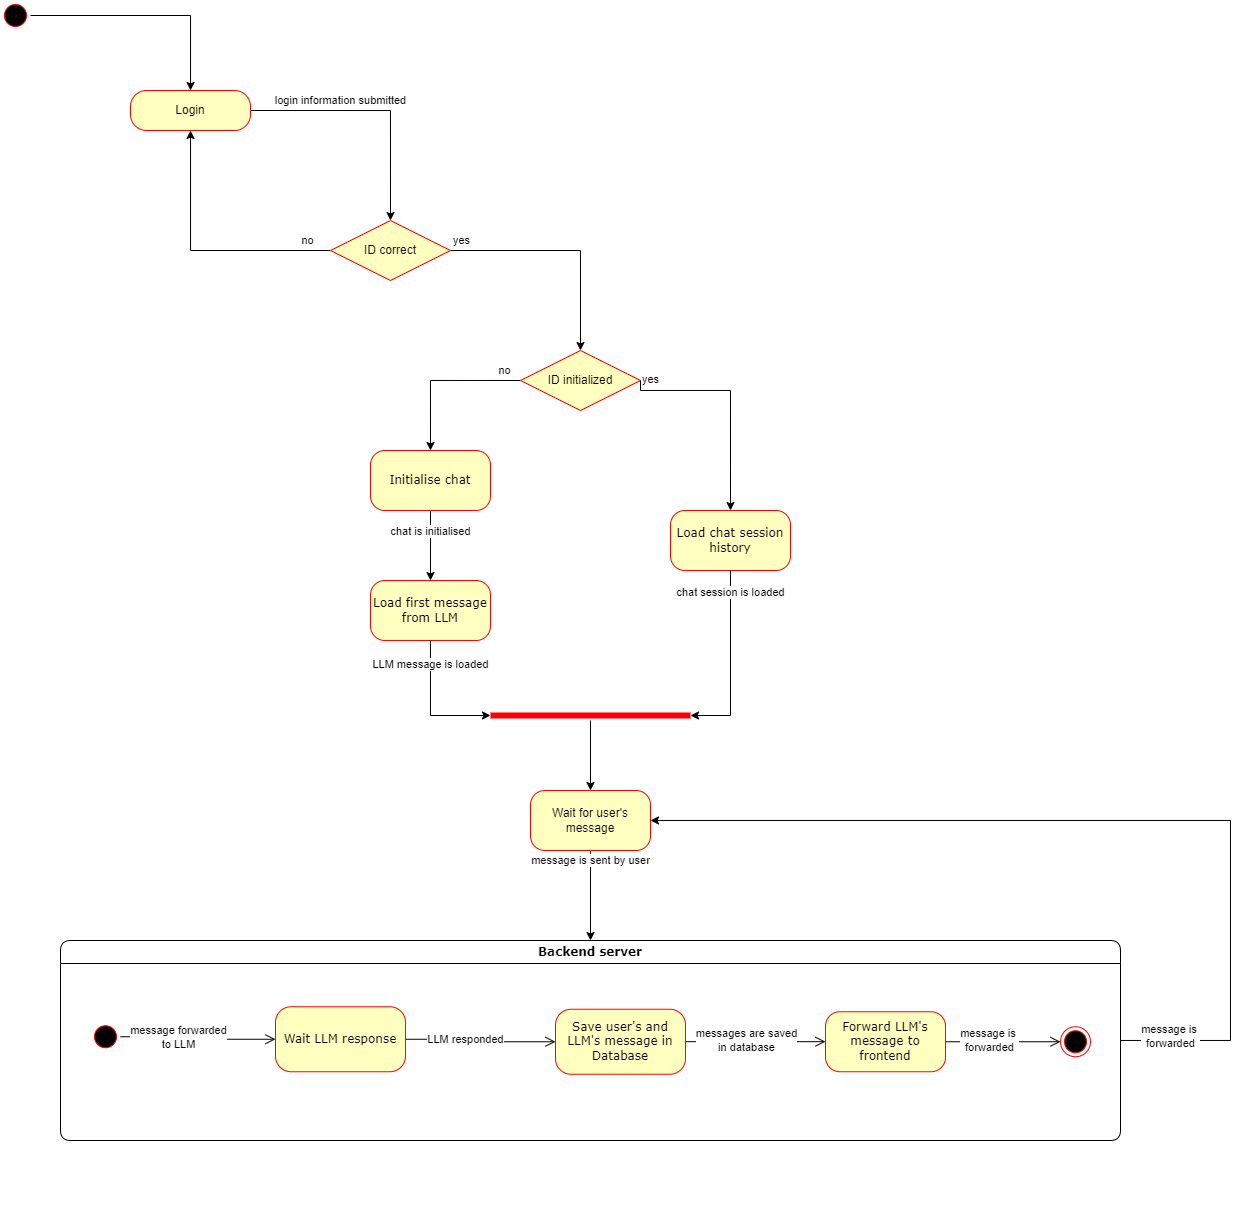
\includegraphics[width=13cm]{state}
    \caption{UML class diagram of the application domain}\label{state}
\end{figure}

\subsection{User Interface}

\subsubsection{Technology Stack}
% \textit{Note: Show mockups of the user interface of the software you develop and their connections / transitions. You can also create a storyboard. \textbf{Important:} Describe the mockups and their rationale in the text.}

\textbf{React.JS}: The application \ac{UI} for this research is primarily built using the popular Javascript framework, React.JS.
React is a free and open-source front-end JavaScript library for building component based \ac{UI}.
This librariy is known for its flexibility and efficiency, which is the main reason why React is being used for this project.
React was crucial for the foundation of the application, making it easier to create responsive and interactive elements.  

\textbf{ Material-UI}: Material-UI, is a React UI library based on Google’s Material Design principles.
This library facilitates the development of \ac{UI} by providing pre-designed components like buttons, forms, and avatars. 
Its seamless integration accelerates development, making it possible  to deliver a polished interface efficiently.

\subsubsection{UI Mockup and Design Process}

Designing the \ac{UI} is a crucial first step in developing an application.
The design should be intuitive and easy to use for the user.
It is even more important for this application, since this application will be used by users from various age groups.
The application should be comfortable to use by every age groups, so that the result is as accurate as possible.
Early in development, \ac{UI} mockups is used before the actual implementation.
This is done to visualize the design and determine whether the design is suitable for the purpose of the application

It is a widely known fact, that an application, especially mobile application such as the one being used for this project, is harder to use for the elderly.
One of the main reasons would be visual impairment that often happen more the older a person gets.
To counteract this, the design of the application is focused on \ac{UI} features, such as bigger interactive elements, high contrast, font selection, spacing, appropriate color choices, and  centralized content.

\begin{figure}[h!]
    \centering
    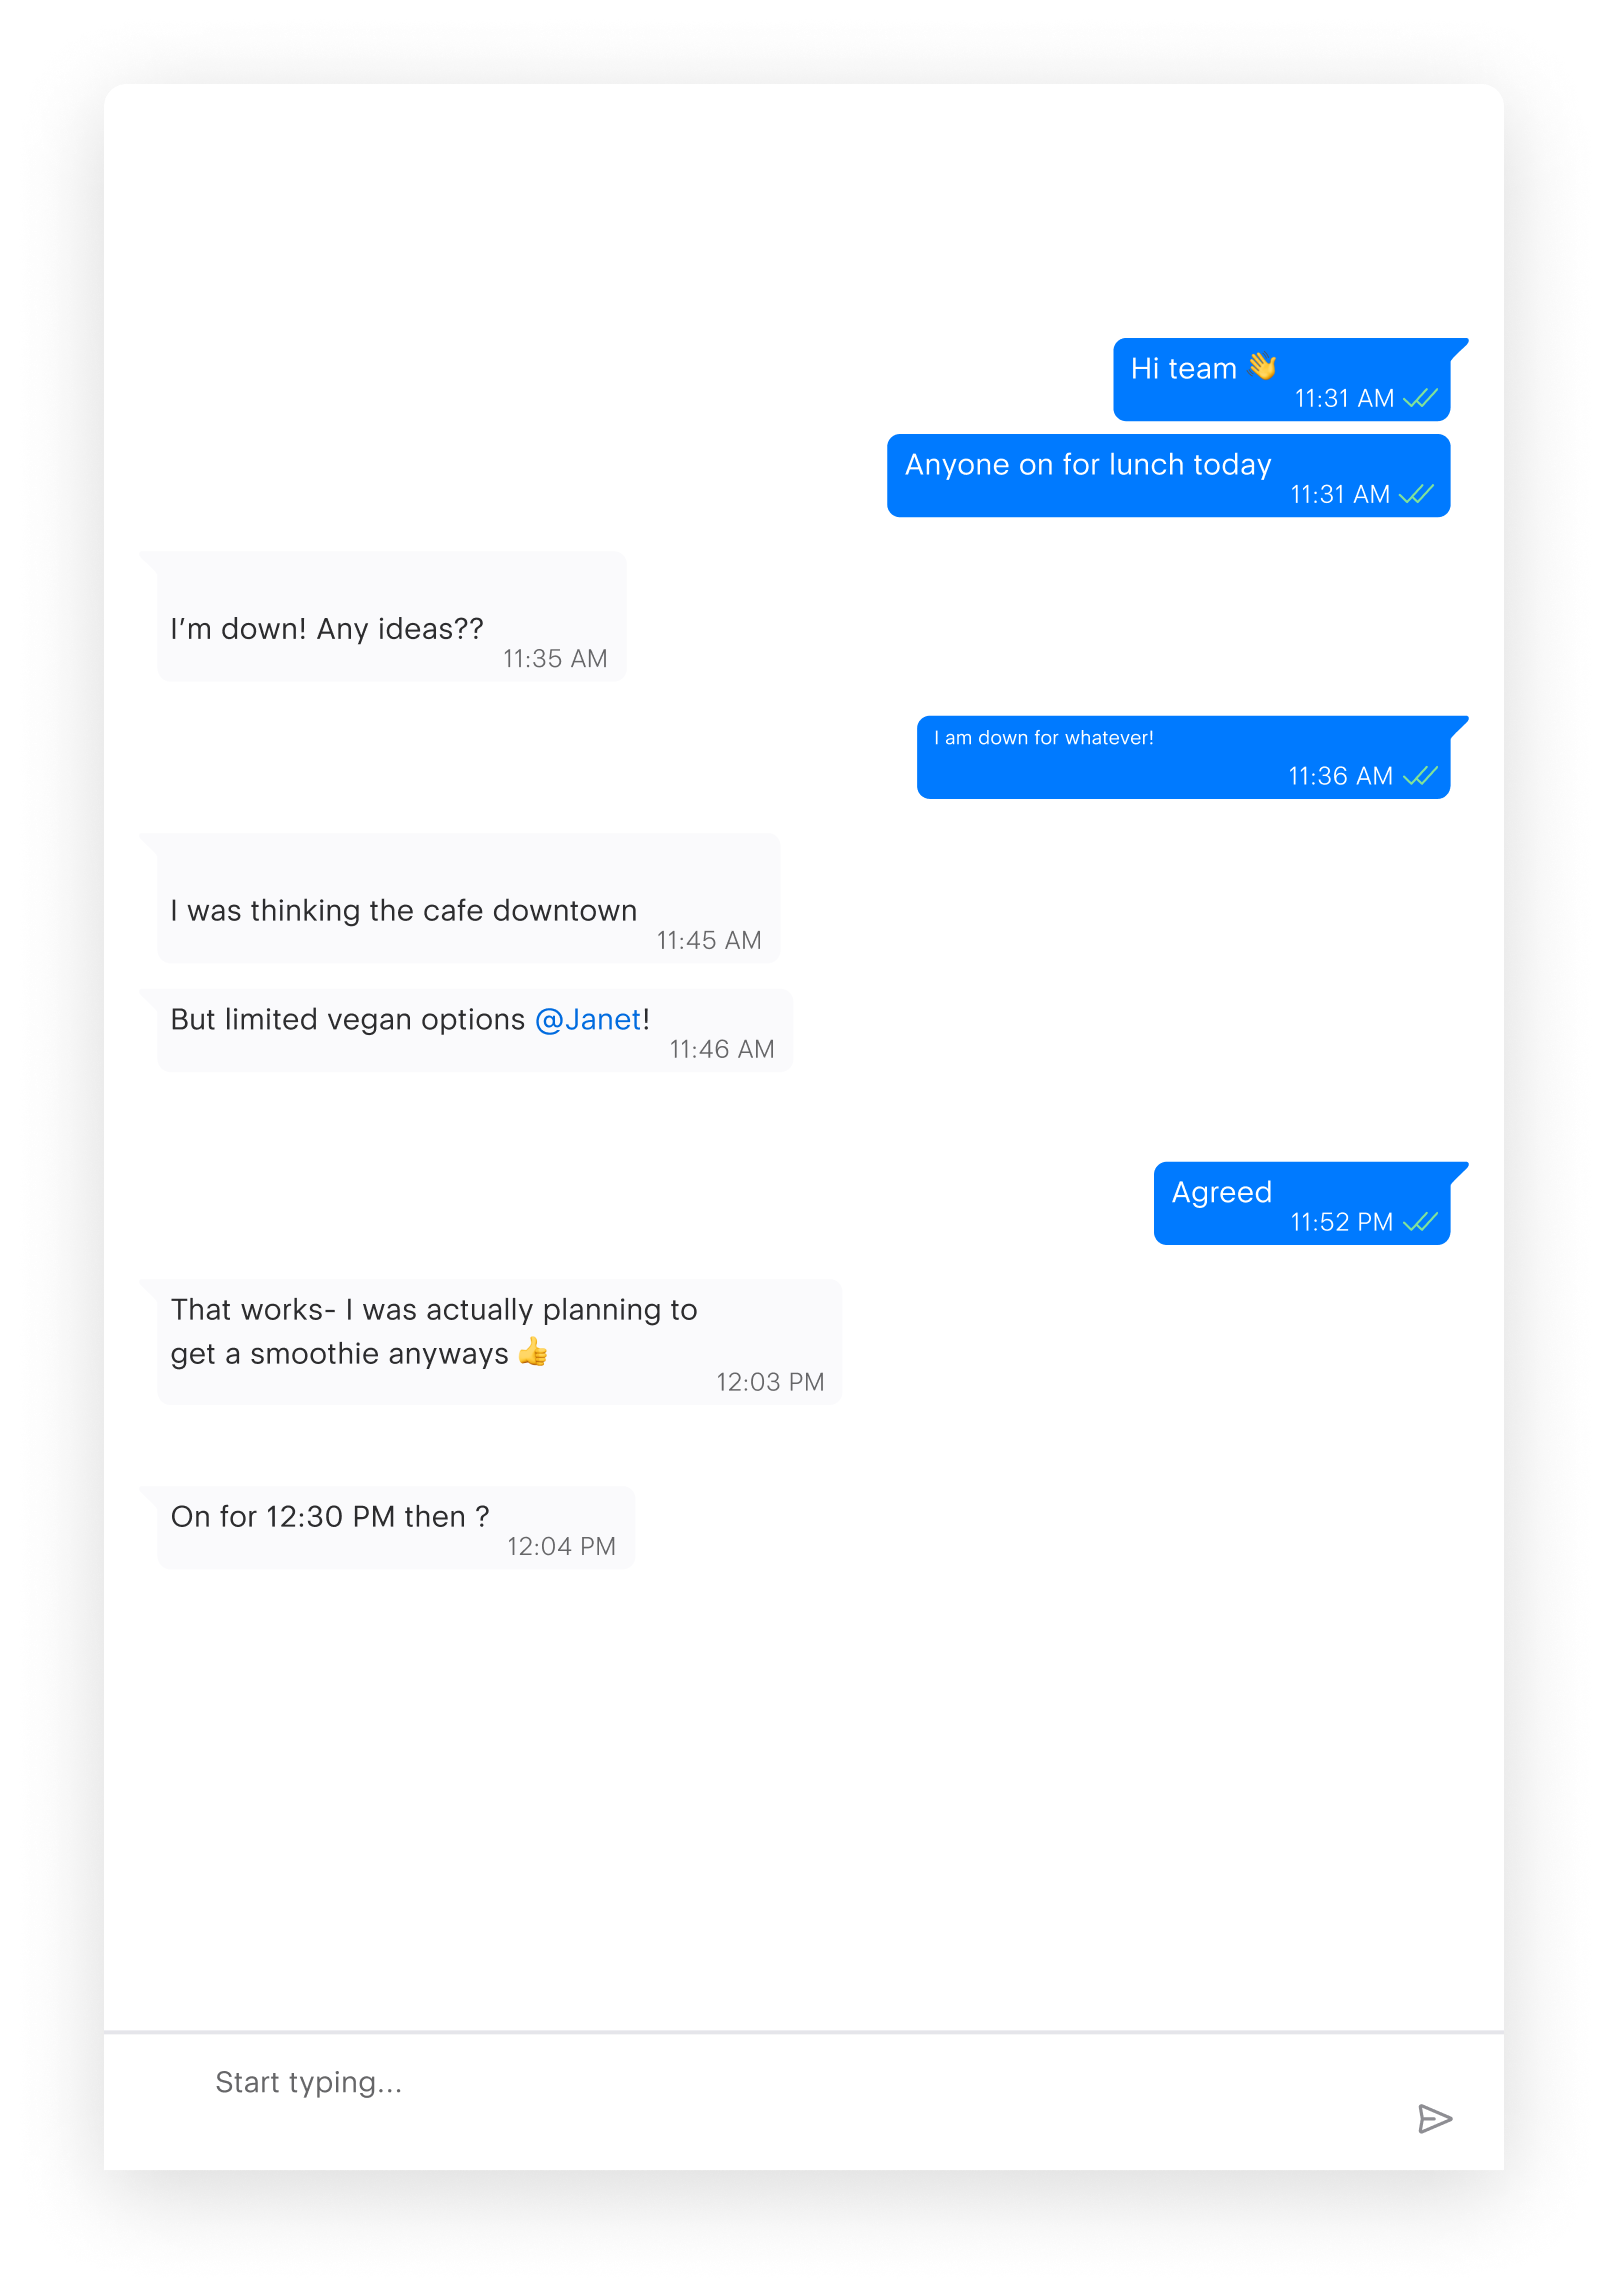
\includegraphics[width=7cm]{message_mockup}
    \caption{\ac{UI} mockup.}\label{mockup}
\end{figure}

The final \ac{UI} mockup did not manage to achieve the intended design.
Figure~\ref{mockup} shows, that the design of the application is not yet user-friendly to the more senior age groups.
The font is too small and the text is too cluttered, are some of the problems that this design has.
However, this mockup design served its purpose as a base design.
Since, as mentioned before, React.JS is known for its flexibility, this problem can easily be solved on the implementation part of the application. 
This mockup serves as a guideline for the layout of the application, with a message input component at the bottom and color-coded text bubbles based on whether the message was from the user or the system.

This adaptation and improvement from the mockup design demonstrated the value of agile development approach.
Changes and adjustments to initial plan are a common accurance in the world of software development.
Many requirements are sometimes missed during planning.
This is one of the main reason that a software should be easily adjustable to ever-changing real world constraints and feedbacks.
While the mockup played a significant role in early planning, the ability to adapt ensured the final product met practical requirements.
 
\subsubsection{Implementation}

Once the mockup is established, the development moves to the implementation phase.

\begin{figure}[h!]
    \centering
    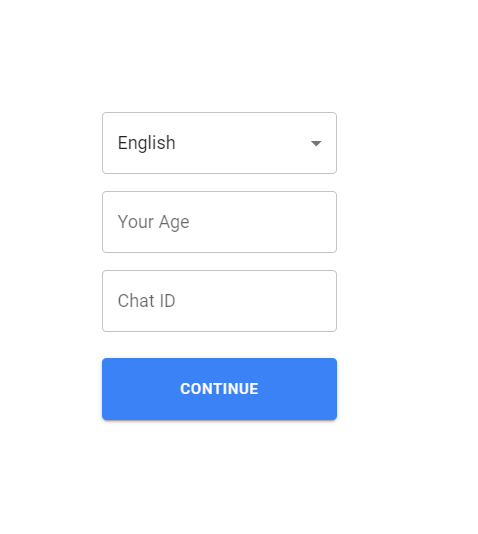
\includegraphics[width=7cm]{login}
    \caption{Login page.}\label{login}
\end{figure}

The first component that is implemented is the login page shown in Figure~\ref{login}.
Login page is important to ensure that each user gets their own chat session and is unable to access a chat session that has ended.
The age of the user is also inputted in this page.
After the login button is clicked, the user is then directed to the chat page.

\begin{figure}[h!]
    \centering
    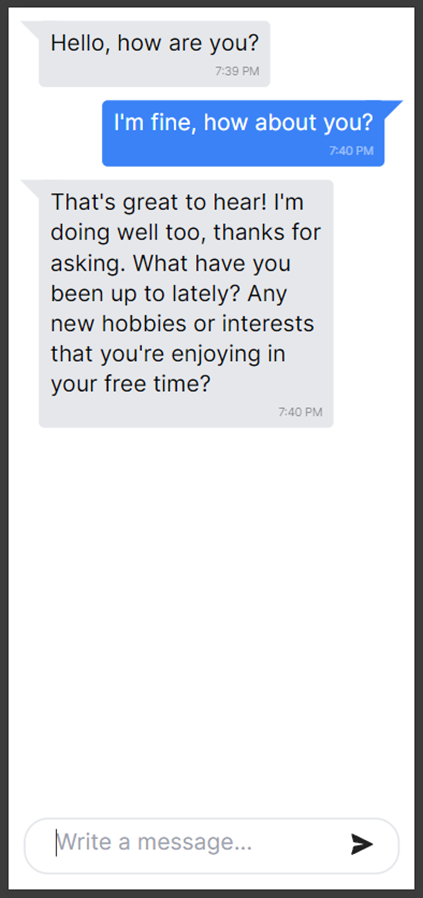
\includegraphics[width=7cm]{simple_app_uncropped}
    \caption{Chat page.}\label{simple_app}
\end{figure}

Figure~\ref{simple_app} shows the chat page.
This chat page is where the user can see the chat history and send a message.
Design of the chat page has been improved, compared to the mockup design.
The font is bigger and the text is more spaced out.
These improvements are done to make the application more user-friendly, especially for the elderly.
To remove the loading speed during the start of the conversation, the first message from the \ac{LLM} is a default message set on the frontend: "Hellow, how are you?".
At the same time, the backend server sends the \ac{LLM} the initial message, which is the prompt.
This allows the \ac{LLM} to load, while the user thinks about the reply for the initial message.

\begin{figure}[h!]
    \centering
    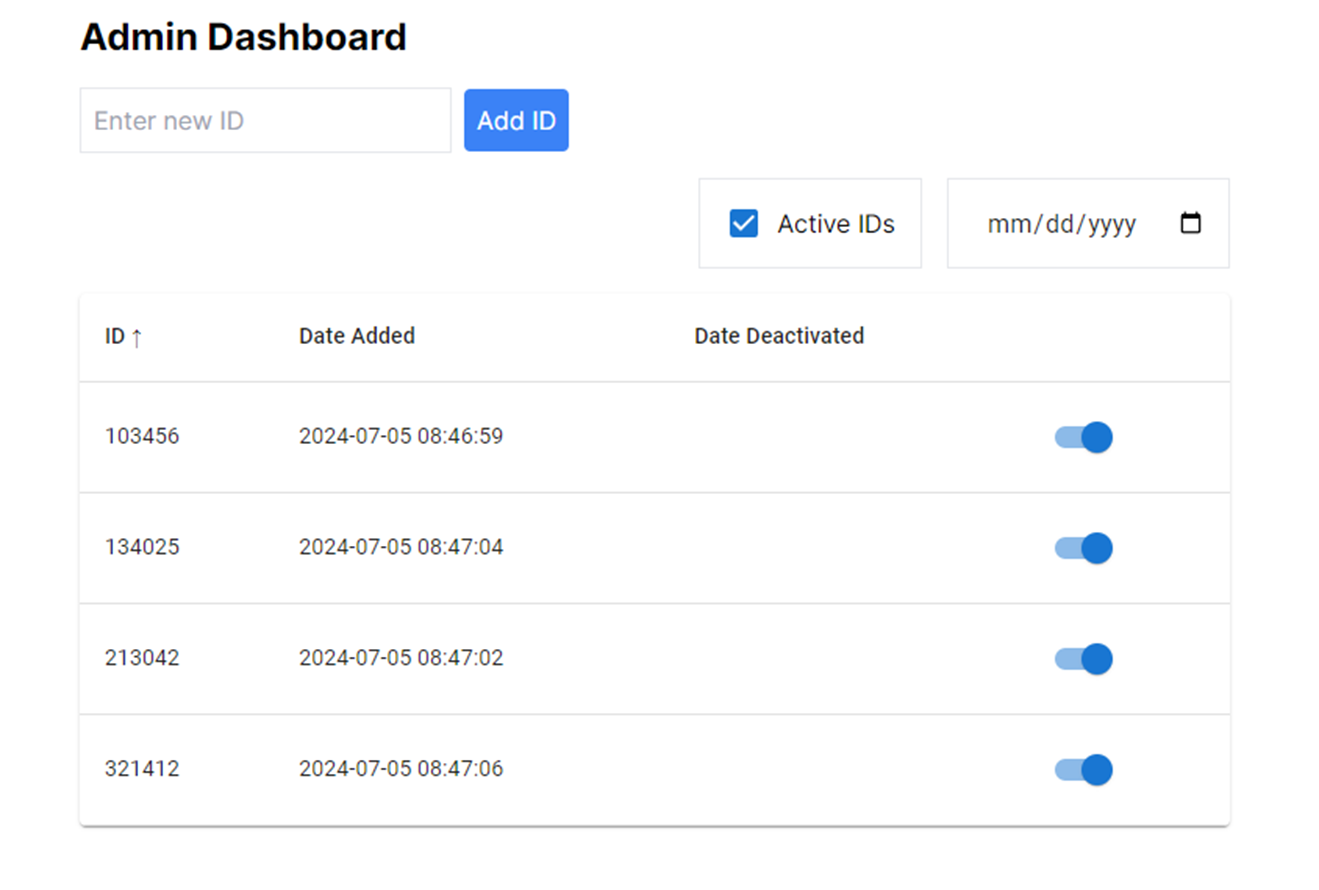
\includegraphics[width=14cm]{admin_dashboard}
    \caption{Admin dashboard page.}\label{admin_dashboard}
\end{figure}

Figure~\ref{admin_dashboard} shows the admin dashboard page.
This page is used by the admin to see ID that has been used by the user.
From this page, the admin can also deactivate a chat session, making it inaccessible.
Some usecases of this feature:
\begin{itemize}
    \item If the user has finished the chat session, the admin can deactivate the chat session.
    \item The admin can give the user a new ID, that has not been accessed before.
    \item The admin has an easy way to see how many conversations have been created and their creation date, without needing to access the database.
    \item With the date filter, the admin can see how many conversations have been created in a certain date.
\end{itemize}
